\documentclass[]{beamer}
\setbeamertemplate{footline}[frame number]
\setbeamertemplate{navigation symbols}{}%remove navigation symbols

\usepackage{url}
\usepackage{cite}
%\usepackage[margin=1in]{geometry}
\usepackage[latin1]{inputenc}
\usepackage{graphicx}
\usepackage{listings}
\usepackage{caption}
\usepackage{subcaption}
\usepackage{paralist}
% uncomment to force centering of captions in IEEE
%\usepackage{subfig}

\usepackage{hyperref}
\hypersetup{
    colorlinks,
    citecolor=black,
    filecolor=black,
    linkcolor=black,
    urlcolor=black
}




\usepackage{tikz}
\usepackage{tikz-er2}
\usetikzlibrary{shapes,arrows}
\usetikzlibrary{positioning}
\usetikzlibrary{shadows}
\tikzstyle{every entity} = [top color=white, bottom color=blue!30,
                            draw=blue!50!black!100, drop shadow]
\tikzstyle{every weak entity} = [drop shadow={shadow xshift=.7ex,
                                 shadow yshift=-.7ex}]
\tikzstyle{every attribute} = [top color=white, bottom color=yellow!20,
                               draw=yellow, node distance=1cm, drop shadow]
\tikzstyle{every relationship} = [top color=white, bottom color=red!20,
                                  draw=red!50!black!100, drop shadow]
\tikzstyle{every isa} = [top color=white, bottom color=green!20,
                         draw=green!50!black!100, drop shadow]
\tikzstyle{decision} = [diamond, draw, fill=blue!20,
    text width=4.5em, text badly centered, node distance=3cm, inner sep=0pt]
\tikzstyle{block} = [rectangle, draw, fill=blue!20,
    text width=5em, text centered, rounded corners, minimum height=4em]
\tikzstyle{edge} = [draw,line,-]
\tikzstyle{line} = [draw, -triangle 45]
\tikzstyle{cloud} = [draw, ellipse,fill=red!20, node distance=3cm,
    minimum height=2em]
\tikzstyle{dot} = [draw, circle, inner sep=1pt, fill=black]
\tikzstyle{db} = [draw,
  shape=cylinder,
  aspect=0.7,
  minimum height=2.5cm,
  minimum width=1.5cm,
  left color=yellow!30,
  right color=yellow!60,
  middle color=yellow!20, % Has to be called after left color and middle color
  outer sep=-0.5\pgflinewidth, % to make sure the ellipse does not draw over the lines
  shape border rotate=90
]


\definecolor{dkgreen}{rgb}{0,0.6,0}
\definecolor{gray}{rgb}{0.5,0.5,0.5}
\definecolor{mauve}{rgb}{0.58,0,0.82}
\lstset{ %
  language=SQL,                % the language of the code
  basicstyle=\scriptsize,           % the size of the fonts that are used for the code
  numbers=none,                   % where to put the line-numbers
  numberstyle=\tiny\color{gray},  % the style that is used for the line-numbers
  stepnumber=2,                   % the step between two line-numbers. If it's 1, each line 
                                  % will be numbered
  numbersep=5pt,                  % how far the line-numbers are from the code
  backgroundcolor=\color{white},      % choose the background color. You must add \usepackage{color}
  showspaces=false,               % show spaces adding particular underscores
  showstringspaces=false,         % underline spaces within strings
  showtabs=false,                 % show tabs within strings adding particular underscores
  frame=single,                   % adds a frame around the code
  rulecolor=\color{black},        % if not set, the frame-color may be changed on line-breaks within not-black text (e.g. comments (green here))
  tabsize=2,                      % sets default tabsize to 2 spaces
  captionpos=b,                   % sets the caption-position to bottom
  breaklines=true,                % sets automatic line breaking
  breakatwhitespace=false,        % sets if automatic breaks should only happen at whitespace
  title=\lstname,                   % show the filename of files included with \lstinputlisting;
                                  % also try caption instead of title
  keywordstyle=\color{blue},          % keyword style
  commentstyle=\color{dkgreen},       % comment style
  stringstyle=\color{mauve},         % string literal style
  escapeinside={\%*}{*)},            % if you want to add LaTeX within your code
  morekeywords={*,...}               % if you want to add more keywords to the set
}

\newcommand{\pad}{\vbox to 20pt{}}


\title[]{Coexist: A database framework for Android and Web clients}
\author[]{Anthony Naddeo \\ adv. Sudarshan Chawathe}
\date{\today}

\usetheme{Berkeley}
\usecolortheme{seagull}

\begin{document}

%--------------------------------------------------------
\begin{frame}
\titlepage
\end{frame}

%--------------------------------------------------------
\section{What is it?}

\begin{frame}
\frametitle{Quick and codeless data management}


\begin{columns}[c]
\column{2in}
Coexist is a framework that allows Android and web clients to perform CRUD operations on a shared database by filling out configuration files.
\column{2in}

\centering
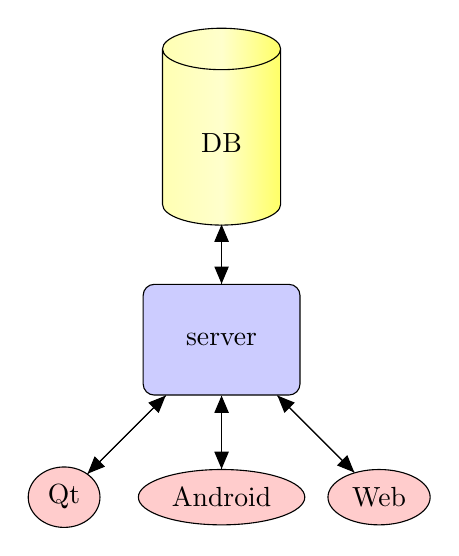
\begin{tikzpicture}[node distance = 2.5cm, auto]
  % Place nodes
  \node [db] (db) {DB};
  \node [block, below of=db] (server) {server};
  
  \node [cloud, below of=server, node distance = 2cm] (client2) {Android};
  \node [cloud, right of=client2, node distance = 2cm] (client1) {Web};
  \node [cloud, left of=client2, node distance = 2cm] (client3) {Qt};

  %pahts
  
  \path [line] (server) -- (db);
  \path [line] (db) -- (server);
  
  \path [line] (client1) -- (server);
  \path [line] (client2) -- (server);
  \path [line] (client3) -- (server);
  \path [line] (server) -- (client1);
  \path [line] (server) -- (client2);
  \path [line] (server) -- (client3);

\end{tikzpicture}
\end{columns}
\end{frame}




%--------------------------------------------------------
\subsection{Importance}

\begin{frame}
\frametitle{Why is this useful?}


\begin{columns}[c]
\column{2in}

\begin{itemize}
\item There is a large overlap between different CRUD focused applications. Having to write a second application to do the same thing as the first, with different data, can be avoided.
\item Enabling mobile (or arbitrary) client types is common enough that it should be done automatically.
\end{itemize}

\column{1in}
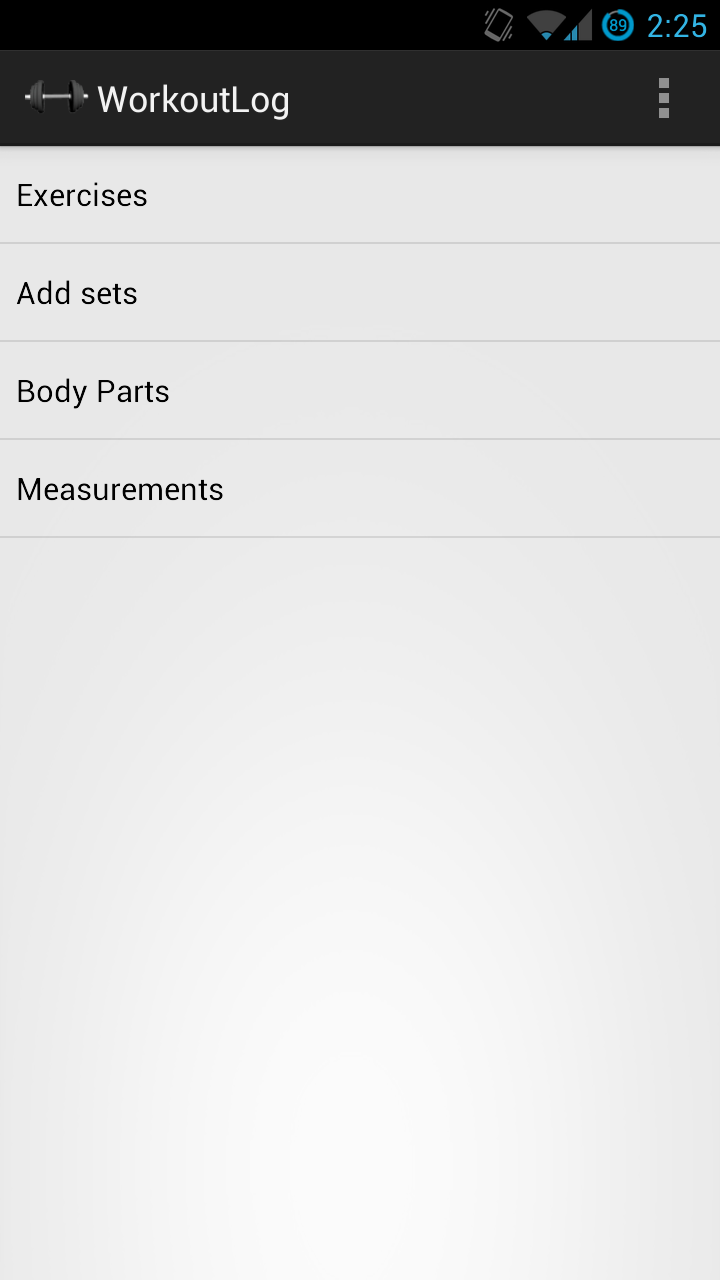
\includegraphics[width=\linewidth]{images/workout.png}
\column{1in}
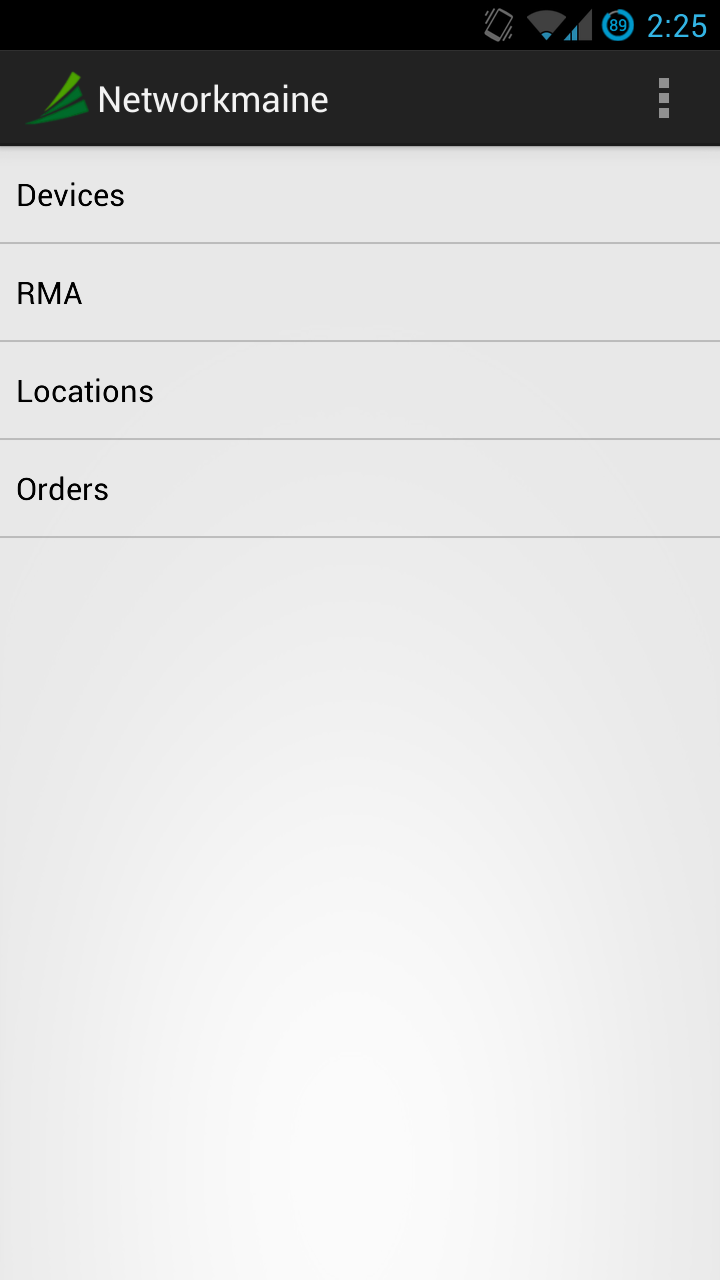
\includegraphics[width=\linewidth]{images/nm.png}
\end{columns}

\end{frame}




%--------------------------------------------------------
\section{Database}

\begin{frame}
\frametitle{How does the database work?}

% needs to support mirroring
% needs to support 

\begin{itemize}
\item The database needs to be mirror-able
\end{itemize}


\end{frame}



%--------------------------------------------------------
\subsection{Implementation}

\begin{frame}
\frametitle{How to support mirroring}
We make use of \textit{metacolumns}: typical SQL columns that are used for some application level purpose.

\begin{columns}[c]
\column{2in}
\scalebox{.8}{
  \begin{tabular}{ l | l | l || l }
  id  & name      & year  & \textit{mod\_ts} \\
  \hline  \hline
  1   & Anthony   & 4     & \textit{0}        \\
  2   & Lucas     & 4     & \textit{10}        \\
  3   & Steven    & 3     & \textit{0}        \\
  4   & Ryan      & 4     & \textit{10}        \\
  \end{tabular}
}
\column{2in}
\small
\begin{itemize}
\item The \texttt{mod\_ts} column contains the most recent update on that tuple
\item Allows the server to give clients missing information when supplied with most recent client side \texttt{mod\_ts}
\end{itemize}
\end{columns}
\end{frame}



%--------------------------------------------------------
\subsection{Motivation}

\begin{frame}
\frametitle{Motivation}
\begin{itemize}
\item The simplest solution.
\item No dependencies.
\end{itemize}

\end{frame}




%--------------------------------------------------------
\section{Server}

\begin{frame}
\frametitle{How does the server work?}

\begin{itemize}
\item The server is designed as an API.
\end{itemize}

\end{frame}







%--------------------------------------------------------
\subsection{Implementation}

\begin{frame}
\frametitle{How to support Synchronization}

\frametitle{Synchronization protocol and API}

There are two simple RESTful function that enable synchronization

\begin{itemize}
\item \texttt{/api/sync} : Request all tuples on the server that are not present on the client.
\item \texttt{/api/schema} : Request the SQL that builds the database.
\end{itemize}

\pad

Normal \texttt{GET} requests can include a representative signature instead. $T$ and $M$ are the concatenation of table names and maximum \texttt{mod\_ts}.
\begin{itemize}
\item \textit{$sha1(version + T + M + username + sha1(password))$}
\end{itemize}

\end{frame}




%--------------------------------------------------------
\subsection{Example}

\begin{frame}
\frametitle{Sample client - server dialog}

\begin{columns}[c]
\column{2in}
Here is a sample conversation between a server and a client who has an out of date schema while attempting to re-sync. \\

\pad

\emph{note:} The application will not require updates for database changes.
\column{2in}
\scalebox{.6}{
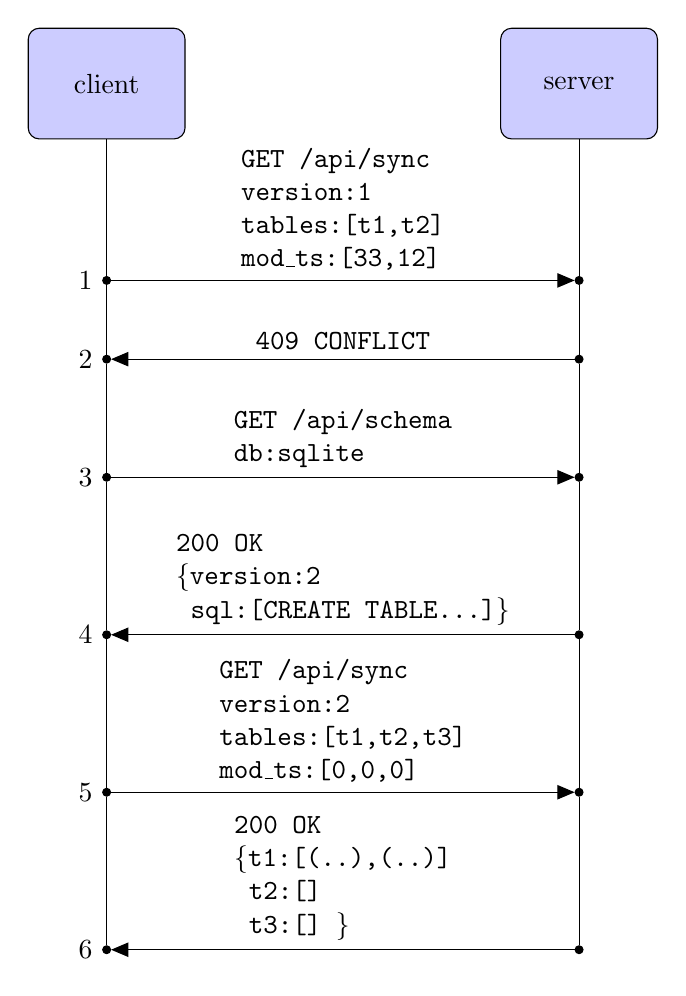
\begin{tikzpicture}[node distance = 2cm, auto]
  % Place nodes
  \node [block] (client) {client};
  \node [block, right of=client, node distance=6cm] (server) {server};
  
  \node [dot, below of=client, node distance=2.5cm, label=180:1] (c1) {};
  \node [dot, below of=server, node distance=2.5cm] (s1) {};
  \path [line] (c1) -- node [above, align=left] {
    \tt\textbf{GET /api/sync} \\ 
    \tt version:1 \\ 
    \tt tables:[t1,t2] \\ 
    \tt mod\_ts:[33,12]}   (s1);
  \path [edge] (client) -- (c1);
  \path [edge] (server) -- (s1);

  \node [dot, below of=c1, node distance=1cm, label=180:2] (c2) {};
  \node [dot, below of=s1, node distance=1cm] (s2) {};
  \path [line] (s2) -- node [above] {\tt\textbf{409 CONFLICT}} (c2);
  \path [edge] (c2) -- (c1);
  \path [edge] (s2) -- (s1);

  \node [dot, below of=c2, node distance=1.5cm, label=180:3] (c3) {};
  \node [dot, below of=s2, node distance=1.5cm] (s3) {};
  \path [line] (c3) -- node [above, align=left] {
    \tt\textbf{GET /api/schema} \\ 
    \tt db:sqlite            } (s3);
  \path [edge] (c2) -- (c3);
  \path [edge] (s2) -- (s3);

  \node [dot, below of=c3, node distance=2cm, label=180:4] (c4) {};
  \node [dot, below of=s3, node distance=2cm] (s4) {};
  \path [line] (s4) -- node [above, align=left] {
    \tt\textbf{200 OK} \\
    \tt\{version:2 \\
    \tt~sql:[CREATE TABLE...]\} } (c4);
  \path [edge] (c3) -- (c4);
  \path [edge] (s3) -- (s4);
    
  \node [dot, below of=c4, node distance=2cm, label=180:5] (c5) {};
  \node [dot, below of=s4, node distance=2cm] (s5) {};
  \path [line] (c5) -- node [above, align=left] {
    \tt\textbf{GET /api/sync} \\ 
    \tt version:2 \\ 
    \tt tables:[t1,t2,t3] \\ 
    \tt mod\_ts:[0,0,0]}   (s5);

  \path [edge] (c5) -- (c4);
  \path [edge] (s4) -- (s5);


  \node [dot, below of=c5, node distance=2cm, label=180:6] (c6) {};
  \node [dot, below of=s5, node distance=2cm] (s6) {};
  \path [line] (s6) -- node [above, align=left] {
    \tt\textbf{200 OK} \\
    \tt \{t1:[(..),(..)] \\
    \tt~t2:[] \\
    \tt~t3:[] \}} (c6);
  \path [edge] (c6) -- (c5);
  \path [edge] (s6) -- (s5);

\end{tikzpicture}
}
\end{columns}


\end{frame}




%--------------------------------------------------------
\subsection{Motivation}

\begin{frame}
\frametitle{Motivation}

\begin{itemize}
\item Simple.
\item A uniform way for accessing the database is needed to allow arbitrary clients to interface independently. 
\item Signatures can be calculated by any client and don't have any [unreasonable] dependencies.
\end{itemize}

\end{frame}


%--------------------------------------------------------
\section{Client}

\begin{frame}
\frametitle{How does the client work?}

\end{frame}




%--------------------------------------------------------
\subsection{Implementation}

\begin{frame}
\frametitle{How does the mobile client work.}


The entire database is mirrored locally.

\vbox to 30pt{}
\begin{columns}[c]
\column{2in}

\begin{itemize}
\item Only dependent on network for posting changes
\item Faster query times than Window or Cache could ever reach
\item Simple to understand
\end{itemize}

\column{2in}
\scalebox{.65}{% 
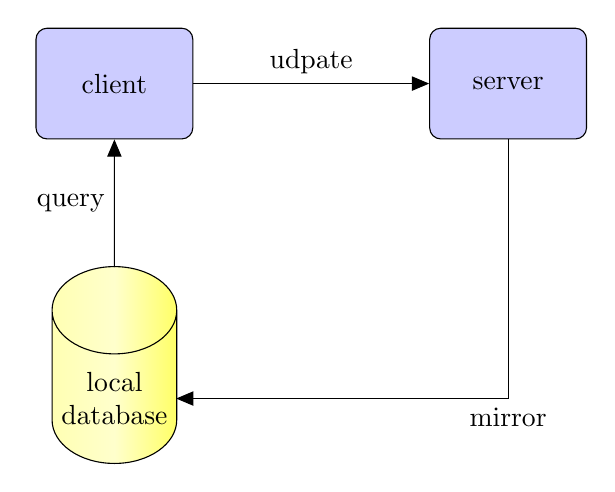
\begin{tikzpicture}[node distance = 2cm, auto]
  % Place nodes
  \node [block] (client) {client};
  \node [block, right of=client, node distance=5cm] (server) {server};
  \node [db, below of=client, node distance=4cm, align=center] (database) {local \\ database};

  % Draw edges
  % Need to align in order to line break
  \path [line] (client) -- node {udpate} (server);
  \path [line] (server) |- node {mirror} (database);
  \path [line] (database) -- node [align=left] {query} (client);
\end{tikzpicture}
}
\end{columns}


\end{frame}


%--------------------------------------------------------

\begin{frame}[fragile]
\frametitle{How does the client know what to request?}


\begin{columns}[c]
\column{2in}
\begin{lstlisting}
[
{"tag":"CAPS05654",
"serial":"000203001056084",
"model":"TCH-17",
"contract number":"none",
"hostname":"USR-Orono1",
"description":"TotalControl17"
},
{"tag":"CAPS05407",
"serial":"72729663",
"model":"7206VXR",
"contract number":"none",
"hostname":"GW-UMF",
"description":"6.SlotChassis"
}
]
\end{lstlisting}
\column{2in}

\begin{lstlisting}
create table Exercises(
  exercise VARCHAR(30) PRIMARY KEY,
  mod_ts DATETIME , -- metacolumn
  deleted INTEGER  -- metacolumn
);

create table Sets(
  name VARCHAR(30),
  exercise VARCHAR(30),
  set_num INTEGER ,
  reps_done INTEGER ,
  weight INTEGER ,
  date_done DATE,
  mod_ts DATETIME, -- metacolumn
  deleted INTEGER -- metacolumn
);

\end{lstlisting}

\end{columns}

\end{frame}


%--------------------------------------------------------
\subsection{Motivation}

\begin{frame}
\frametitle{Motivation}

\begin{itemize}
\item Coexist was designed with mobile clients in mind, and offline-readability as a feature.
\item All queries can be performed locally and avoid network bottleneck.
\item After initial sync, only missing rows are ever downloaded. 
\end{itemize}

\end{frame}




%--------------------------------------------------------
\section{Deployment}

\begin{frame}[fragile]
\frametitle{How does deployment work?}

\begin{columns}[c]
\column{1.6in}
Tentatively, a conf file must be filled out. I have made a tool that will download and compile the latest version of Coexist and its clients according to this.
\column{2.5in}
\begin{lstlisting}

; Android stuff
name=Workoutlog
image=logo.png
notification=notification.png
package=com.domain
api=http://domain.com:/api/

; Server stuff
version=1
user=
pass=
db=
host=localhost
dbms=mysql

create_dir=ui 
schema_dir=sql

\end{lstlisting}

\end{columns}


\end{frame}




%--------------------------------------------------------
\section{Future}

\begin{frame}
\frametitle{What needs to be done?}

\begin{itemize}
\item Add more client types (Qt, Desktop Java etc.)
\item Support more client features (i.e. Barcode scanning on mobile clients.)
\item Create tools to automate the configuration.
\end{itemize}

\end{frame}


%--------------------------------------------------------
\section{Thanks}

\begin{frame}
\frametitle{I would like to thank}

My advisor, Sudarshan Chawathe

\end{frame}




\end{document}
